\chapter{Localization on a clustered graph}
\label{ch:localization}

% Added 2026-09-25.  Numbers from statmech/probe/anderson.py (scan); figure and
% tables from figs/anderson.py.  See book/extensions.md.

Every message so far has been a probability, a field, a survey or a count.
This chapter carries the recursion with a message that is a Green's
function, on the problem that has been the Bethe lattice's since
\citet{abouchacra1973}: a quantum particle hopping on a graph with random
site energies, which is localised or extended depending on energy and
disorder \citep{anderson1958}. The occasion is a specific one.
\citet{tonetti2025} test, on the $K+1=3$ Bethe lattice, the proposal of
\citet{filoche2012} that the mobility edge is the percolation threshold of
a classical landscape computed from the same Hamiltonian, and find that the
two lines do not coincide and are of different universality classes. They
attribute the discrepancy to interference, which lives on loops, of which
the tree has none. A chygraph with triangles has the shortest loops, and
treats them exactly. So the question this chapter asks is the one their
paper leaves: what do loops do to the two lines, and to the gap between
them.

\section{The resolvent as a message}
\label{sec:resolvent}
\index{Green's function|textbf}
\index{Schur complement|textbf}
\index{Anderson model|textbf}

The Anderson model on a graph is $\hat H=\sum_{i}\epsilon_{i}\,|i\rangle\langle
i|-t\sum_{\langle ij\rangle}\bigl(|i\rangle\langle j|+|j\rangle\langle
i|\bigr)$, with $\epsilon_{i}$ independent and uniform on $[-W/2,W/2]$ and
$t=1$ throughout. Everything about localisation is in the resolvent
$\mathcal{G}(z)=(\hat H-z)^{-1}$ at $z=E-\mathrm{i}0^{+}$: its diagonal
element is the local density of states, and its imaginary part vanishes
site by site in the localised phase and does not in the extended one.

On a tree the diagonal element obeys the two steps of
Sec.~\ref{sec:twosteps} with an edge for a complex,
\begin{equation}
  \mathcal{G}_{ii}^{-1}=\epsilon_{i}-z-\sum_{a\ni i}\Sigma_{a\to i},
  \qquad
  \Sigma_{a\to i}=t^{2}\,\mathcal{G}_{k\to i},
  \label{eq:treeG}
\end{equation}
where $\mathcal{G}_{k\to i}$ is the diagonal element at the other end of the
edge with $i$ removed, computed from $k$'s other edges by the same rule.
These are Eqs.~(3) and~(4) of \citet{tonetti2025}, and Eq.~(S11) of their
supplement. The down step is the interior of the complex --- a single
number, $t^{2}\mathcal{G}$ --- and the up step is a sum over complexes,
which is the linearity of the self-energy in the branches.

On a chygraph the up step is unchanged and the down step is a matrix
inverse. Let complex $a$ have members $i$ and $J=a\setminus i$, let $A_{J}$
be the adjacency of the clique among $J$, and let $\Sigma_{J\to a}$ be the
diagonal matrix of the members' cavity self-energies from their other
complexes. Then the self-energy the complex transmits to $i$ is a Schur
complement,
\begin{equation}
  \Sigma_{a\to i}(z)=t^{2}\,\mathbf{1}^{\mathsf T}
  \bigl[(\epsilon_{J}-z)-t A_{J}-\Sigma_{J\to a}\bigr]^{-1}\mathbf{1},
  \label{eq:schur}
\end{equation}
which is the interior of the complex summed exactly, in the only sense a
resolvent can be summed: every path from $i$ into the complex and back out
to $i$, through any of its members any number of times, with the members'
own branches folded into $\Sigma_{J\to a}$. At cardinality two $J=\{k\}$ and
Eq.~\eqref{eq:schur} is $t^{2}/(\epsilon_{k}-z-\Sigma_{k\to a})$, which is
Eq.~\eqref{eq:treeG}. For a triangle it is a $2\times2$ inverse in closed
form,
\begin{equation}
  \Sigma_{a\to i}=t^{2}\,\frac{m_{1}+m_{2}+2t}{m_{1}m_{2}-t^{2}},
  \qquad m_{j}=\epsilon_{j}-z-\Sigma_{j\to a},
  \label{eq:triangleG}
\end{equation}
with the $2t$ in the numerator the loop: the path from $i$ to $j_{1}$ to
$j_{2}$ and back, which is what the tree cannot have.

\begin{figure}[t]
\centering
\begin{tikzpicture}
% A triangle complex a = {i, j1, j2}. The two members j carry the self-energies
% of their other complexes (drawn as stubs); what a transmits to i is the Schur
% complement over {j1, j2}, and the loop j1-j2 is the term the tree lacks.
\node[hub] (i) at (0,0) {};
\node[lb,anchor=north] at (0,-0.16) {$i$};
\node[nd] (j1) at (-1.05,1.55) {};
\node[nd] (j2) at (1.05,1.55) {};
\node[lb,anchor=east] at (-1.20,1.55) {$j_{1}$};
\node[lb,anchor=west] at (1.20,1.55) {$j_{2}$};
\draw[lnk] (i)--(j1) (i)--(j2);
\draw[lnk,line width=1.0pt] (j1)--(j2);
\node[tb,anchor=south] at (0,1.66) {$t$: the loop};
\begin{scope}[on background layer]
  \node[cx,fit=(i)(j1)(j2)] (A) {};
\end{scope}
% stubs: the members' other complexes, folded into their cavity self-energies
\draw[lnk,black!35] (j1)--++(-0.55,0.75) (j1)--++(-0.85,0.15);
\draw[lnk,black!35] (j2)--++(0.55,0.75) (j2)--++(0.85,0.15);
\node[lb,anchor=south east] at (-1.25,2.30) {$\Sigma_{j_{1}\to a}$};
\node[lb,anchor=south west] at (1.25,2.30) {$\Sigma_{j_{2}\to a}$};
% the transmitted self-energy
\draw[msg] (0.20,0.95) -- (0.10,0.30);
\node[lb,anchor=west] at (0.30,0.62) {$\Sigma_{a\to i}$};
\node[lb,anchor=west,align=left] at (2.35,0.75)
  {\emph{down}, Eq.~\eqref{eq:triangleG}:\\
   invert the $2\times2$ block\\
   $\begin{pmatrix} m_{1} & -t\\ -t & m_{2}\end{pmatrix}$,\\
   $m_{j}=\epsilon_{j}-z-\Sigma_{j\to a}$,\\
   and sum its entries.\\
   The $-t$ off the diagonal\\
   is the loop.};
\end{tikzpicture}
\caption{\textbf{The interior of a complex, for a resolvent.} A triangle
$a=\{i,j_{1},j_{2}\}$: the members $j$ carry the self-energies of their
other complexes, and what $a$ transmits to $i$ is the Schur complement of
Eq.~\eqref{eq:schur} over $\{j_{1},j_{2}\}$, every path from $i$ into the
complex and back, the hop $j_{1}j_{2}$ included. On an edge there is no
such hop and the block is a number, which is the tree recursion.}
\label{fig:schur}
\end{figure}

Two things follow. On any chygraph whose incidence structure is a tree
Eq.~\eqref{eq:schur} is exact, and Sec.~\ref{sec:loc-checks} confirms it to
$10^{-15}$ against direct inversion. And the cost is polynomial in the
cardinality --- a $(c-1)\times(c-1)$ inverse rather than a sum over $2^{c}$
states --- so the hard ceiling of Sec.~\ref{sec:notdone} does not apply to
this model: a complex of thirty members is a $29\times29$ matrix.

\paragraph{The ensembles.} The Bethe lattice is the regular chygraph with
every atom in three edges. Beside it this chapter puts the regular chygraphs
in which every atom belongs to $s$ single edges and $t$ triangles, written
$(s,t)$, so that $(3,0)$ is \citeauthor{tonetti2025}'s lattice and
$(1,1)$ has the same degree with one of the three neighbour pairs closed
into a loop; at degree four, $(4,0)$, $(2,1)$ and $(0,2)$. Holding the
degree fixed is Sec.~\ref{sec:threads}'s rule: the comparison is between
graphs with the same number of neighbours per site, differing in whether
those neighbours are neighbours of each other. The population dynamics
carries two populations of self-energies, one per cardinality, and an atom
left out of an edge draws $s-1$ edge messages and $t$ triangle messages,
left out of a triangle $s$ and $t-1$: the excess bracket of
Fig.~\ref{fig:themap}, once more.

The spectrum of the pure hopping problem on $(s,t)$ has a bottom $e_{\min}$
that the uniform fixed point of Eq.~\eqref{eq:schur} locates --- the largest
$E$ below which a real solution exists --- and an isolated eigenvalue
$-t(s+2t)$ carried by the uniform vector, as on any regular graph
\citep{biroli2010}. With disorder the bottom of the spectrum is
$E_{\min}(W)=e_{\min}-W/2$ once that lies below the isolated eigenvalue,
which for $(3,0)$ is $W>0.34$ and agrees with \citeauthor{tonetti2025}'s
$W_{\min}$; every disorder used here is above it. Table~\ref{tab:andersonwc}
lists $e_{\min}$: $-2\sqrt2$ and $-2\sqrt3$ for the two trees, which is the
check, and lower for the triangle ensembles, since a triangle's lowest
eigenvalue is $-2t$ against an edge's $-t$.

\section{The landscape, by linearity}
\label{sec:landscape}
\index{localization landscape|textbf}

The Localization Landscape is $u=(\hat H-E_{\min})^{-1}\mathbf{1}$, the
solution of a linear equation with the spectrum shifted to make the
operator positive, and \citet{arnold2016} show that $1/u$ is an effective
confining potential: eigenstates of $\hat H-E_{\min}$ at energy $E'$ live
where $1/u\le E'$. Its $i$th component is a row sum of the resolvent at
real $z=E_{\min}$, where nothing needs regularising, and on the Bethe
lattice \citeauthor{tonetti2025} write it as $u_{i}=\mathcal{G}_{ii}\eta_{i}$
with $\eta_{i}=1+t\sum_{k}\mathcal{G}_{k\to i}\eta_{k\to i}$, their Eqs.~(5)
to~(7): the row sum of a branch is the row sum of its root times what the
root transmits.

The same linearity carries it to a complex. With $M_{a}$ the real matrix
inverted in Eq.~\eqref{eq:schur} at $z=E_{\min}$ and $\eta_{J\to a}$ the
vector of the members' cavity row sums,
\begin{equation}
  \begin{aligned}
  \eta_{a\to i}&=t\,\mathbf{1}^{\mathsf T}M_{a}^{-1}\,\eta_{J\to a},\\
  \eta_{i}&=1+\sum_{a\ni i}\eta_{a\to i},
  \qquad
  u_{i}=\mathcal{G}_{ii}(E_{\min})\,\eta_{i},
  \end{aligned}
  \label{eq:landscape}
\end{equation}
where $\eta_{j\to a}=1+\sum_{b\ni j,\,b\ne a}\eta_{b\to j}$. On an incidence
tree this is exact, and on random instances of $3000$ atoms it reproduces
the direct solve to a relative error of $10^{-8}$ on the trees and
$3\times10^{-3}$ on the densest triangle ensemble, the residue being the
long loops of the instance. The landscape is smooth: $u$ at neighbouring
atoms is strongly correlated, because both are dominated by the same
branches, and Sec.~\ref{sec:lltperc} has to carry that correlation or it
gets the percolation threshold wrong.

\section{Landscape percolation as a dependent layer}
\label{sec:lltperc}
\index{dependent layer}

The LLT proposal is that a state at energy $E'=E-E_{\min}$ is extended iff
the set $\{i:u_{i}\ge1/E'\}$ percolates. That is site percolation with an
occupation that is not independent from site to site but a function of a
cavity field, which is the dependent-layer construction of
Sec.~\ref{sec:joint} with a threshold rule of the kind Sec.~\ref{sec:groupcontagion}
met: here the field is continuous, so the transition is continuous, and
\citeauthor{tonetti2025} find it mean-field, $\gamma=1$, on the tree. On the
chygraph the map is Part~II's,
\begin{equation}
  \begin{aligned}
  p_{j\to a}&=\theta\bigl(u_{j}-1/E'\bigr)
  \Bigl[1-\prod_{b\ni j,\,b\ne a}(1-p_{b\to j})\Bigr],\\
  p_{a\to i}&=1-\prod_{j\in J}(1-p_{j\to a}),
  \end{aligned}
  \label{eq:lltmap}
\end{equation}
the second line because a clique's members are all adjacent to $i$, so $i$
reaches the infinite cluster through $a$ if any other member does. The
landscape $u_{j}$ in the first line is the full one --- it includes the
complex $a$ through which $j$ is reached, since $u$ is a property of the
site --- and the message $\Sigma_{a\to j}$, $\eta_{a\to j}$ that completes
it is computed from the other members' cavity data in the same draw.
Every population element is therefore a triple $(\Sigma,\eta,p)$ generated
from one cavity draw. Generating $p$ separately, with the same marginals,
moves the threshold by a tenth (Fig.~\ref{fig:andersonmech}), which is the
smoothness of $u$ at work: open sites are found next to open sites.

The threshold is located by the growth rate of a small $p$ under
Eq.~\eqref{eq:lltmap}, renormalised each generation, which is the
linearisation of Sec.~\ref{sec:threshold} done numerically because the
$\theta$ makes the joint law awkward to write. On $(3,0)$ at $W=1.5$ the
threshold is $E'_{c}=0.473$, that is $E_{c}^{\mathrm{perc}}=E_{\min}+E'_{c}=-3.106$
at the bottom of the band, which by the symmetry of the tree's spectrum is
$3.106$ at the top against \citeauthor{tonetti2025}'s $3.165$, two per cent
apart. The triangle ensembles are not bipartite and their spectra are not
symmetric, so everything here is done at the bottom of the band and
compared there.

\section{The mobility edge as a stability line}
\label{sec:mobility}
\index{mobility edge|textbf}
\index{de Almeida--Thouless line}

The localised phase is the fixed point of Eq.~\eqref{eq:schur} at real
$z=E$: every message real, the imaginary parts zero. The extended phase is
where that fixed point is unstable to an infinitesimal imaginary part, and
the criterion is the one this book has used for every transition, the
linearised map at the trivial fixed point, applied to the imaginary parts
with the real parts frozen at their distribution. Writing $M_{a}$ for the
real matrix of Eq.~\eqref{eq:schur} and $v=M_{a}^{-1}\mathbf{1}$,
\begin{equation}
  \operatorname{Im}\Sigma_{a\to i}=t^{2}\sum_{j\in J}v_{j}^{2}
  \sum_{b\ni j,\,b\ne a}\operatorname{Im}\Sigma_{b\to j},
  \label{eq:imlinear}
\end{equation}
a linear map with positive random weights: $t^{2}\mathcal{G}_{k\to i}^{2}$ on
an edge, which is \citeauthor{tonetti2025}'s Eq.~(S14), and
$t^{2}[(m_{2}+t)/(m_{1}m_{2}-t^{2})]^{2}$ and its partner on a triangle.
Because the weights have heavy tails the right growth rate is not that of
the mean but of a fractional moment: the localised phase is stable iff
$\lambda(\beta)<1$ for some $\beta\in(0,1)$, where $\lambda(\beta)$ is the
growth factor per generation of $\langle(\operatorname{Im}\Sigma)^{\beta}\rangle$
under Eq.~\eqref{eq:imlinear}, and the transition is where
$\min_{\beta}\lambda(\beta)=1$ \citep{abouchacra1973}. That minimum sits at
$\beta=1/2$ on the tree by a symmetry of the kernel, and the population
estimate here scans $\beta$ over $0.4$ to $0.6$. This is the de
Almeida--Thouless argument of Sec.~\ref{sec:atline} with a fractional
power in place of the square: a perturbation of random size, transmitted
with a random factor, whose typical growth decides.

The estimate is biased by the population. At the band centre of $(3,0)$,
where the transition is at $W_{c}=18.17$ \citep{tikhonov2019,parisi2019},
$\lambda(1/2)$ at $W=18$ is $0.967$, $0.977$ and $0.986$ with $2\times10^{5}$,
$10^{6}$ and $3\times10^{6}$ elements, rising towards one as the heavy tail
of the moment is sampled better, and the threshold read from
$10^{6}$ elements is a few per cent low. At the bottom of the band the
bias is smaller: $(3,0)$ at $W=1.5$ gives $E_{c}^{\mathrm{loc}}=-3.106$
against \citeauthor{tonetti2025}'s $-3.152$. The comparisons that matter
below are between ensembles at the same population, where the bias is
common.

\section{What loops do}
\label{sec:loops}

Three figures carry the result; the numbers behind them are cached with
the probe's results and \code{figs/\allowbreak localization.\allowbreak py}
prints them. Both lines are energies at the
bottom of the band, a state being extended for $E>E_{c}^{\mathrm{loc}}$ and
the landscape percolating for $E>E_{c}^{\mathrm{perc}}$; the gap
$E_{c}^{\mathrm{perc}}-E_{c}^{\mathrm{loc}}$ is positive where the LLT misses
extended states and negative where it invents them. Seven of the thirty
points were computed twice from independent populations: the percolation
threshold repeats to $0.002$ and the mobility edge to $0.003$ at $W=1.5$
and $0.03$ at $W=6$, which are the error bars.

\paragraph{The lines, measured from the band edge.}
Figure~\ref{fig:anderson} plots both lines as their distance above
$E_{\min}$, which removes the $-W/2$ that every line shares and leaves what
the disorder does. Three things are visible at once. The mobility edge
climbs away from the band edge roughly linearly in $W$ on every ensemble:
the localised skin at the bottom of the band thickens with disorder. The
percolation line climbs faster on every ensemble, so the two cross where
they are going to cross and separate thereafter; on the degree-three tree
they start together, a gap of $0.006$ at $W=1.5$ against
\citeauthor{tonetti2025}'s $0.013$, which is their small-disorder
agreement, and on the degree-four tree the percolation line starts below
the mobility edge and crosses it near $W=4.3$, which is the crossing they
report. And the triangle ensembles lie above the trees on the percolation
line and on top of them on the mobility edge: at degree three the two
mobility edges are within $0.1$ of each other up to $W=3$ while the two
percolation lines are $0.1$ to $0.7$ apart. Whatever the loops do, they do
it to the landscape.

\paragraph{The gap.} Figure~\ref{fig:andersongap} is the difference, and
it is the chapter's result in one panel. At every disorder the gap
increases with the number of triangles at fixed degree, and it does so by
moving the crossing to weaker disorder: $W\approx4.3$ on the degree-four
tree, $3.0$ with one triangle per site, $1.7$ with two. Above the crossing
the ordering never changes --- $0.27$, $0.49$, $0.75$ at $W=6$ and $1.3$,
$1.5$, $1.9$ at $W=12$ --- and at degree three the cactus opens a gap of
$0.20$ where the tree has none. Then the cactus does something the tree
does not. At $W=9$ its curve stops: the imaginary parts decay at every
energy, the whole band is localised, and the landscape still percolates,
at $E_{c}^{\mathrm{perc}}=-2.58$ and, at $W=12$, $-2.29$. That is not a shift
of a line but a line drawn through a band in which nothing is extended,
and the LLT has no way of knowing it.

\paragraph{Why the cactus localises first.} Figure~\ref{fig:andersoncentre}
gives the reason, at the band centre where it is cleanest: the growth rate
$\lambda(1/2)$ of Eq.~\eqref{eq:imlinear} against disorder for the five
ensembles, the transition being where it crosses one.
Table~\ref{tab:andersonwc} lists the crossings: $17.4$ on the degree-three
tree, $8.6$ on the cactus at the same degree; $32.3$, $26.2$ and $18.1$ at
degree four as edges become triangles. The last number is within a unit of
the degree-three tree's, and that is the mechanism in one line. What the
imaginary recursion propagates is amplitude along walks that never turn
back, and a triangle spends two of a site's neighbours on each other: a
walk that leaves through the edge of the cactus and enters a triangle has
one way on where the tree offered two, so the number of such walks grows
as $\sqrt2$ per step instead of $2$, and two triangles per site give
$\sqrt2\cdot\sqrt2=2$, the degree-three tree's growth. Fewer walks, less
interference to sustain an extended state, and the graph localises at a
disorder the tree shrugs off. The landscape does not know this. It is a
static, positive solution of a shifted linear problem, for which the loop
is the $2t$ in the numerator of Eq.~\eqref{eq:triangleG}, a slightly
larger self-energy and a slightly smoother $u$, and nothing about walks.

\paragraph{The two mechanisms, checked.} Figure~\ref{fig:andersonmech}
shows the two criteria at work. On the left, $\lambda(1/2)$ against energy
at $W=3$ for the tree and the cactus: a smooth crossing of one, at
$0.78$ above the band edge on the tree and $1.02$ on the cactus, which is
the mobility edge as a stability line, with the cactus's localised skin
thicker by a quarter of a unit. On the right, the percolation growth
factor against $E'$ on the tree at $W=1.5$, with the $(\Sigma,\eta,p)$
triple drawn jointly and with $p$ drawn from separate members of the
population: the threshold moves from $E'=0.47$ to $0.52$, a tenth, which
is what the smoothness of $u$ is worth, and a calculation that treats the
landscape as independent site by site gets the LLT's own prediction wrong.

\paragraph{What this says about the proposal.} \citeauthor{tonetti2025}
found the two transitions apart on the tree and conjectured that loops,
which carry the interference the landscape cannot see, would be where
they part company. On these graphs loops do part them, in one direction
and by one route: every triangle moves the percolation line towards the
band centre and leaves the mobility edge nearly where it was, so the
landscape's picture of allowed regions that connect at a threshold is a
worse guide to where the states are the more the graph is clustered,
until on the degree-three cactus it percolates through a band with no
extended state in it. The one mitigating case is the weak-disorder
crossing on the degree-four graphs, where triangles bring the crossing
down to $W=1.7$ and the lines are briefly together; that is the regime of
the three-dimensional agreement of \citet{filoche2012}, and it is narrow.

\begin{figure}[t]
\centering
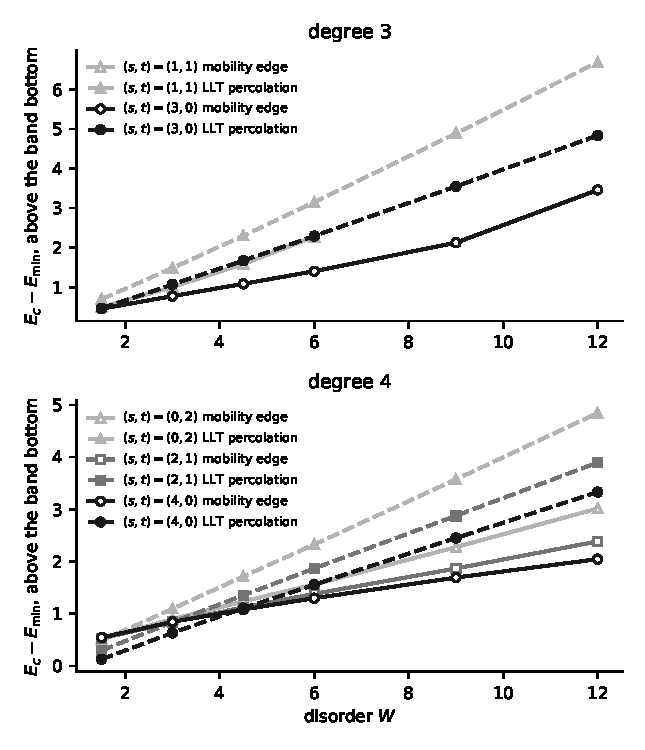
\includegraphics[width=\linewidth]{figs/fig-anderson.pdf}
\caption{\textbf{Two lines above the band edge.} The mobility edge
$E_{c}^{\mathrm{loc}}$ (solid, open markers) and the landscape percolation
threshold $E_{c}^{\mathrm{perc}}$ (dashed, filled), each measured from the
bottom of the spectrum $E_{\min}(W)$, against disorder, for regular
chygraphs with $s$ edges and $t$ triangles per site at degree three (top)
and four (bottom). A mobility-edge curve that stops is a band that has
localised entirely. Generated by \code{figs/\allowbreak
localization.\allowbreak py} from \code{statmech/\allowbreak
probe/\allowbreak anderson.\allowbreak py}.}
\label{fig:anderson}
\end{figure}

\begin{figure}[t]
\centering
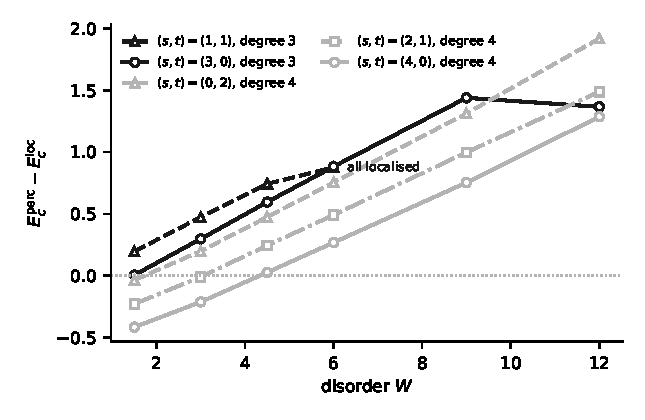
\includegraphics[width=\linewidth]{figs/fig-anderson-gap.pdf}
\caption{\textbf{The gap.} $E_{c}^{\mathrm{perc}}-E_{c}^{\mathrm{loc}}$
against disorder for the five ensembles, dark for degree three and light
for degree four: positive where the landscape misses extended states,
negative where it invents them. At fixed degree the gap grows with the
number of triangles at every disorder, and the cactus $(1,1)$ leaves the
plot at $W=9$ because its band has localised entirely while its landscape
still percolates. Generated by \code{figs/\allowbreak
localization.\allowbreak py}.}
\label{fig:andersongap}
\end{figure}

\begin{figure}[t]
\centering
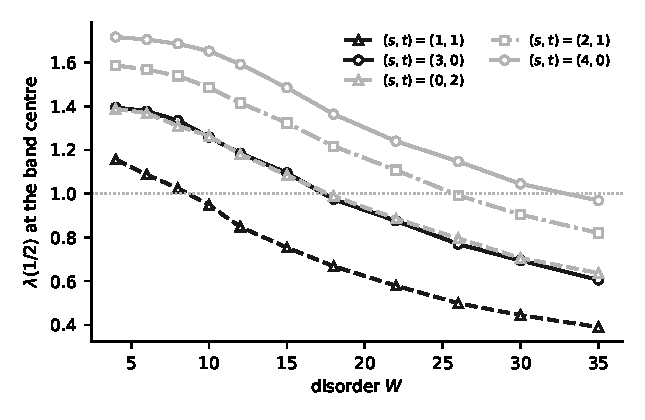
\includegraphics[width=\linewidth]{figs/fig-anderson-centre.pdf}
\caption{\textbf{Where the band centre localises.} The growth rate
$\lambda(1/2)$ of the linearised imaginary recursion, Eq.~\eqref{eq:imlinear},
at $E=0$ against disorder; the band centre is extended above the dotted
line. Two triangles per site, $(0,2)$, localise where three edges per
site, $(3,0)$, do, which is the $\sqrt2$ per triangle of the walks that
carry interference. Populations of $3\times10^{5}$; the crossings in
Table~\ref{tab:andersonwc} use $10^{6}$. Generated by \code{figs/\allowbreak
localization.\allowbreak py}.}
\label{fig:andersoncentre}
\end{figure}

\begin{figure}[t]
\centering
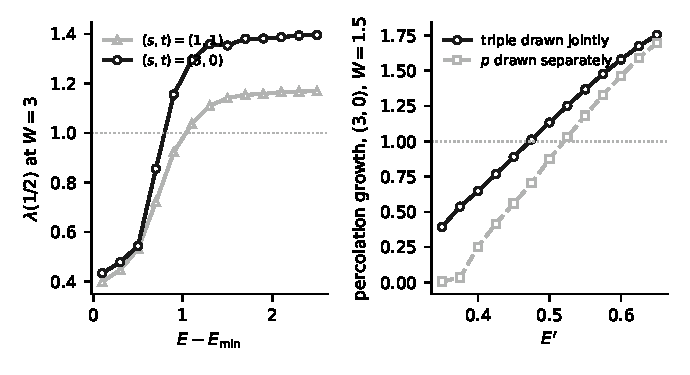
\includegraphics[width=\linewidth]{figs/fig-anderson-mechanism.pdf}
\caption{\textbf{The two criteria at work.} Left: $\lambda(1/2)$ against
energy above the band edge at $W=3$ on the degree-three tree and cactus;
the mobility edge is the crossing of one. Right: the growth factor of the
landscape percolation message against $E'$ on the tree at $W=1.5$, with
the $(\Sigma,\eta,p)$ triple drawn jointly, as Sec.~\ref{sec:lltperc}
requires, and with $p$ drawn from separate members of the population; the
threshold is the crossing of one and the difference is the smoothness of
$u$. Generated by \code{figs/\allowbreak localization.\allowbreak py} from
\code{statmech/\allowbreak probe/\allowbreak anderson.\allowbreak py},
mode \code{side}.}
\label{fig:andersonmech}
\end{figure}

\begin{table}[t]
\centering\small
\begin{tabular}{ccrr}
\hline\hline
$(s,t)$ & degree & band bottom & $W_{c}$ at $E=0$\\
\hline
$(1,1)$ & 3 & $-2.9655$ & $8.6$\\
$(3,0)$ & 3 & $-2.8284$ & $17.4$\\
$(0,2)$ & 4 & $-3.8285$ & $18.1$\\
$(2,1)$ & 4 & $-3.6477$ & $26.2$\\
$(4,0)$ & 4 & $-3.4641$ & $32.3$\\
\hline\hline
\end{tabular}

\caption{\textbf{Band bottoms and band-centre critical disorder.} The
pure-hopping band bottom $e_{\min}$ from the uniform fixed point of
Eq.~\eqref{eq:schur}, and the disorder $W_{c}$ at which the band centre
localises, from $\min_{\beta}\lambda(\beta)=1$ with $10^{6}$ elements; the
tree value $17.4$ sits four per cent below the $18.17$ of
\citet{tikhonov2019}, which is the population bias of
Sec.~\ref{sec:mobility}. Generated by \code{figs/\allowbreak
localization.\allowbreak py}.}
\label{tab:andersonwc}
\end{table}

\section{Conclusions}
\label{sec:loc-conclusions}

A Green's function is a message like any other in this book: the recursion
is the two steps, the interior of a complex is summed exactly, and what
changes is that the sum is a Schur complement, polynomial in the
cardinality where every other chapter paid $2^{c}$. On that footing the
two problems of \citet{tonetti2025} close on any chygraph of cliques, and
on regular graphs of edges and triangles they answer the question their
paper raised. Loops separate the landscape percolation line from the
mobility edge rather than joining them: the percolation line moves towards
the band centre with every triangle, the mobility edge scarcely moves, the
gap grows with the triangle count at fixed degree and disorder, and on the
degree-three cactus the landscape percolates through a band in which
nothing is extended. The mechanism is that loops halve the growth of the
walks that carry interference while adding a term to a static denominator,
and a static object cannot tell the difference.

What is not done is the critical behaviour, which \citeauthor{tonetti2025}
find to differ between the two transitions on the tree; nothing here
computes an exponent, and the lines are located to a few hundredths, the
mobility edge less well than the threshold. The population bias on the mobility edge is a few
per cent and common to the comparisons made. And the ensembles are
regular; a chygraph of the maximal cliques of a real network, with the
degree and cardinality distributions of Chapter~\ref{ch:data}, is the same
calculation with populations of populations by layer and is not run here.

\section{Checks}
\label{sec:loc-checks}

\code{figs/\allowbreak localization.\allowbreak py} runs, before it draws
anything: the cavity of Eq.~\eqref{eq:schur} against direct inversion of
$\hat H-z$ on finite incidence trees of edges and triangles, to $10^{-15}$;
the pure-hopping band bottoms of $(3,0)$ and $(4,0)$ against $-2\sqrt2$ and
$-2\sqrt3$. \code{statmech/\allowbreak probe/\allowbreak anderson.\allowbreak
py check} adds the random instances: on $600$ atoms the error of the
cavity resolvent falls from $4\times10^{-2}$ to $6\times10^{-6}$ as the
imaginary part of $z$ goes from $0.2$ to $3$, which is what long loops do
and short ones do not, and the landscape agrees with the direct solve to
$10^{-8}$ on the trees. The two benchmarks against \citet{tonetti2025} and
the band-centre $W_{c}$ are the tests from outside the formalism, and the
population bias is quoted rather than hidden. Everything in this chapter is
at the level of the mobility edge and the threshold; nothing here computes
a critical exponent, and \citeauthor{tonetti2025}'s finding that the two
transitions differ in class is taken from them, not reproduced.
